\documentclass[UTF-8]{ctexbeamer}
\usecolortheme{seahorse}

\usepackage{multimedia}
\usepackage{listings}
\usepackage{minted}
\usepackage[normalem]{ulem}

\title{How NOT to Rust}

\author{喵喵}
\date{2021.10}

\begin{document}
\begin{frame}
  \titlepage
  \begin{center}
    
\includegraphics[width=.1\textwidth]{assets/float.png}
  \end{center}
\end{frame}

\begin{frame}
  \frametitle{How NOT to Rust}

  本来想用的标题是 \texttt{A Brief, Incomplete, and Mostly Wrong History of Rust}\footnote{\url{http://james-iry.blogspot.com/2009/05/brief-incomplete-and-mostly-wrong.html}}。

  \pause
  \vspace{1em}

  但是喵喵写 Slide 毫无灵感\dots

  \begin{figure}
    \includegraphics<2>[width=0.25\textwidth]{assets/avatar.jpg}
    \includegraphics<3>[width=0.5\textwidth]{assets/avatarWD40.png}
    \only<2>{\caption{呼呼喵喵}}
    \only<3>{\caption{精神喵喵!!}}
  \end{figure}
\end{frame}

\begin{frame}
  \frametitle{How NOT to Rust}

  来聊聊 Rust 的历史。(其实大多数是喵喵的 Rant)

  \pause

  这个 Talk 包括:
  \begin{itemize}
    \item Rust Overview!
    \item Rust 的各种 Joke
  \end{itemize}

  这个 Talk 不包括:
  \begin{itemize}
    \item Rust 详细入门,请查看 The Rust Programming Language
    \item Rust 详细语义,请查看 The Rust Language Reference
    \item 讲者存在 Rust 深刻知识的任何可能。
  \end{itemize}

  \pause

  喵喵刚刚入门 Rust,请爱护喵喵!
\end{frame}

\begin{frame}
  \frametitle{快速 Rust 入门}

  Rust 和 \texttt{C(|++), Java(|Script), Python, LISP, \dots} 有什么不同?

  \pause
  \vspace{1em}

  \begin{itemize}
    \item Algebraic Data Types
    \item \texttt{crate} and \texttt{module}
    \item Polymorphism: Generic + Trait
    \item (The dreaded) Lifetime / \texttt{borrowck}
  \end{itemize}
\end{frame}

\begin{frame}[fragile]
  \frametitle{ADT: Algebraic Data Types}

  \begin{minted}{rust}
// KV DB, Client -> Server conn payload
enum KVPayload {
  Close,
  Get(String),
  Put {
    key: String,
    value: String,
    expire: Datetime,
  },
}
  \end{minted}

  \pause
  \vspace{1em}
  Disjoint sum over products!
\end{frame}

\begin{frame}[fragile]
  \frametitle{Generic over type}

  \begin{minted}{rust}
    enum SingleOrVec<T> {
      Single(T),
      Vec(Vec<T>),
    }
  \end{minted}
\end{frame}

\begin{frame}[fragile]
  \frametitle{Generic over type...?}

  Heap allocation are bad.

  \pause

  \begin{minted}{rust}
    enum SingleOrArray<T, const N: usize> {
      Single(T),
      Array([T; N]),
    }
  \end{minted}

  \pause
  \vspace{1em}

  Const generics (rfcs\#2000)
\end{frame}

\begin{frame}[fragile]
  \frametitle{Module-level encapsulation}

  Crate = Node/Go/Python package (sort of)

  功能集合,例如:\texttt{serde} 提供了序列化、反序列化相关的基础设施。

  \pause
  \vspace{1em}

  Module = Java package (sort of)

  实现单元,“可见性“的边界。例如:\texttt{serde::ser} 包含序列化 (Serialize) 相关的声明和实现。

  \pause
  \vspace{1em}

  \begin{minted}{rust}
mod data;
pub use data::{Input, Output};
  \end{minted}
\end{frame}

\begin{frame}[fragile]
  \frametitle{Abusing modules}

  \texttt{library/std/src/os/mod.rs:}

  \begin{minted}[breaklines]{rust}
// unix
#[cfg(not(all(
    doc,
    any(
        all(target_arch = "wasm32", not(target_os = "wasi")),
        all(target_vendor = "fortanix", target_env = "sgx")
    )
)))]
#[cfg(target_os = "hermit")]
#[path = "hermit/mod.rs"]
pub mod unix;
  \end{minted}
\end{frame}

\begin{frame}[fragile]
  \frametitle{C style preprocessor?}

  \pause

  \only<1-2>{With procedure macro?}
  \only<3>{\sout{With procedure macro?}}
  \begin{minted}{rust}
preprocess!{
  #ifdef PLATFORM_WINDOWS
    // Do something
  #else
    // Do something else
  #endif
}
  \end{minted}

  \pause
  \vspace{1em}

  Please don't.
  
\end{frame}

\begin{frame}
  \frametitle{Polymorphism}

  \begin{itemize}
    \item Composition over Inheritance {\tiny{设计模式!}}
    \item Trait: 描述一个接口
    \pause
    \item Generic: 使用 Trait 的静态派发
    \item Trait Objects: 使用 Trait 的动态派发
  \end{itemize}
\end{frame}

\begin{frame}[fragile]
  \frametitle{Polymorphism, Cont.}
  \begin{minted}{rust}
trait Monoid {
  // "Member functions"
  fn product(&self, other: &Self) -> Self;
  // "Static functions"
  fn identity() -> Self;
  fn is_commutative() -> bool;
}

trait Group: Monoid {
  fn inverse(&self) -> Self;
  // Default impl
  fn is_abelian() -> bool {
    return Self::is_commutative();
  }
}
  \end{minted}
\end{frame}

\begin{frame}[fragile]
  \frametitle{Polymorphism, Cont.}

  \begin{minted}{rust}
struct Cyclic<const N: usize>(usize);

impl<const N: usize> Monoid for Cyclic<N> {
    fn product(&self, ano: &Self) -> Self {
        let inner = self.0;
        let anoinner = ano.0;
        return Self((self.0 + ano.0) % N)
    }
    fn identity() -> Self { Self(0) }
    fn is_commutative() -> bool { true }
}
    
  \end{minted}

  

\end{frame}

\begin{frame}[fragile]
  \frametitle{Polymorphism, Cont.}

  \begin{minted}{rust}
fn subgroup_by<G>(gen: G) -> Vec<G>
  where G: Group + Eq + Clone
{
  let mut cur = gen.clone();
  let mut result = Vec::new();
  loop {
    result.push(cur.clone());
    cur = cur.product(gen);
    if cur == gen {
      return result;
    }
  }
}
  \end{minted}
\end{frame}

\begin{frame}[fragile]
  \frametitle{Polymorphism, Cont.}

  \begin{minted}{rust}
    let trait_obj: &dyn Group = &group;
  \end{minted}

  \pause
  \vspace{1em}

  VTable with fat pointer

  \pause
  \vspace{1em}
  
  \pause
  \begin{minted}{rust}
  let boxed_fn: Box<dyn Fn(usize) -> usize> =
    Box::new(
        |input: usize| -> usize {
            input * 2
        }
    );
  \end{minted}
\end{frame}

\begin{frame}[fragile]
  \frametitle{Polymorphism... ?}

  \begin{minted}{rust}
trait Trait {}
fn generic_fn<T: Trait + ?Sized>() {
  println!("{}", size_of::<&dyn Trait>()); // -> 16
  println!("{}", size_of::<&T>());         // -> 8
}
  \end{minted}
\end{frame}

\begin{frame}[fragile]
  \frametitle{Polymorphism... ?}

  \begin{minted}{rust}
trait Trait {}
fn generic_fn<T: Trait + ?Sized>() {
  println!("{}", size_of::<&dyn Trait>()); // -> 16
  println!("{}", size_of::<&T>());         // -> 16
}

fn main() {
  generic_fn::<dyn Trait>();
}
  \end{minted}
\end{frame}

\begin{frame}[fragile]
  \frametitle{Why Traits?}
  
  \pause

  \only<2>{没有“基类对象”,没有“菱形继承”。}
  \only<3->{没有“基类对象”,\sout{没有“菱形继承”。}}

  \pause

  \begin{minted}{rust}
trait Common {}
trait SpecA {}
trait SpecB {}

impl<T: SpecA> Common for T { }
impl<T: SpecB> Common for T { }
  \end{minted}
  
  \pause
  \vspace{1em}

  Rust \sout{(尝试)} 禁止这件事情。
  \begin{itemize}
    \item Orphan rule
    \pause
    \item "Strictly more specified"
  \end{itemize}
\end{frame}

\begin{frame}[fragile]
  \frametitle{Why Traits (More Solid)}

  \begin{minted}{rust}
trait Common {}
trait SpecA {}
trait SpecB {}

impl<T: SpecA> Common for T { }
impl<T: SpecB + SpecA> Common for T { }
  \end{minted}

  \pause
  \vspace{1em}

  You'll need
  \begin{minted}{rust}
#![feature(specialization)]
  \end{minted}

  See also: RFC 1210: Specialization

  \pause
  \vspace{1em}

  "Chalk"
\end{frame}

\begin{frame}
  \frametitle{impl Trait for (A, B, C)}

  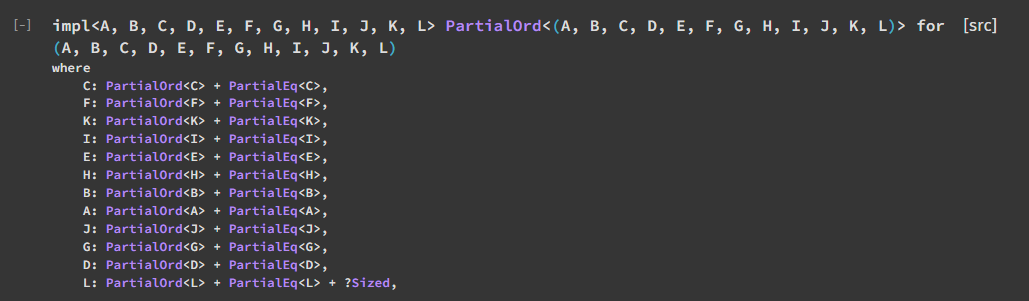
\includegraphics[width=\textwidth]{assets/tuple.png}
\end{frame}

\begin{frame}
  \frametitle{What about array?}

  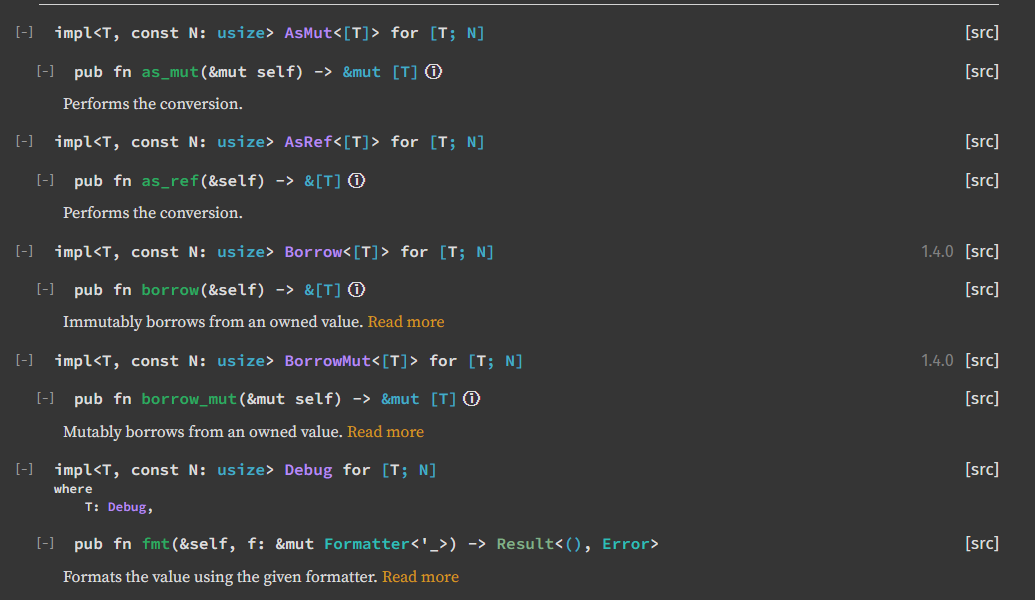
\includegraphics[width=\textwidth]{assets/array-good.png}
\end{frame}

\begin{frame}[fragile]
  \frametitle{What about array....???}

  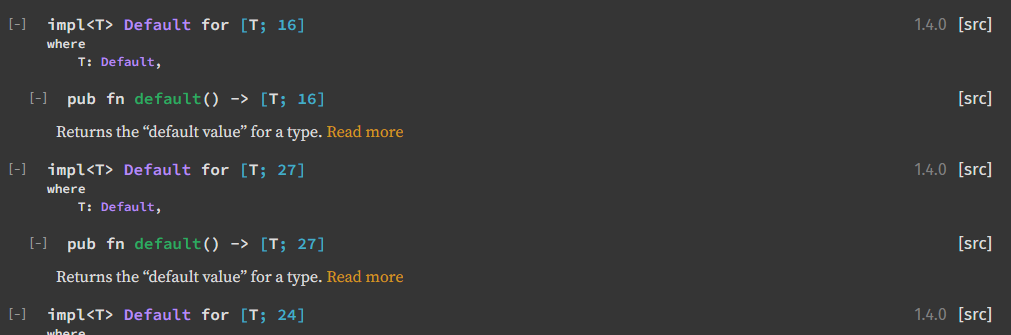
\includegraphics[width=\textwidth]{assets/array-bad.png}

  \pause
  \vspace{1em}

  \begin{minted}{rust}
impl<T: const N: usize> Default for [T; N]
  where T: Default;
  \end{minted}

  \pause

  \begin{minted}{rust}
impl<T> Default for [T; 0];
  \end{minted}
\end{frame}

\begin{frame}[fragile]
  \frametitle{Trait: Operator Overloading}

  \pause

  \begin{minted}{rust}
struct Point(f64, f64);
impl Add for Point {
  type Output = Point;
  fn add(self, rhs: Point) -> Point {
    let Point(sx, sy) = self;
    let Point(rs, ry) = rhs;
    Point(sx + rs, sy + ry)
  }
}
  \end{minted}
\end{frame}

\begin{frame}[fragile]
  \frametitle{Trait: Operator Overloading, Cont.}
  \begin{minted}{rust}
#[lang = "add"]
pub trait Add<Rhs = Self> {
  // ...
}
  \end{minted}
  \pause

  \begin{minted}{rust}
impl Add for usize {
  type Output = usize;

  #[inline]
  #[rustc_inherit_overflow_checks]
  fn add(self, rhs: usize) -> usize {
    self + rhs
  }
}
  \end{minted}
\end{frame}

\begin{frame}[fragile]
  \frametitle{Let's look at \texttt{Box}}

  \begin{minted}{rust}
impl<T: ?Sized, A: Allocator> Deref for Box<T, A> {
  type Target = T;

  fn deref(&self) -> &T {
      &**self
  }
}
  \end{minted}

  \pause
  \vspace{1em}

  Box is a "primitive"
\end{frame}

\begin{frame}[fragile]
  \frametitle{But wait...}

  \begin{minted}{rust}
struct MeowBox<T> {
  ptr: *mut T,
}

impl<T> MeowBox<T> {
  fn new(e: T) -> MeowBox<T> {
    unsafe {
      let space = alloc();
      ptr::write(space, e);
    }
    MeowBox<T> {
      ptr: space
    }
  }
}
  \end{minted}
\end{frame}

\begin{frame}[fragile]
  \frametitle{Box is special}

  \begin{minted}{rust}
let old_school: ~usize = ~10;
let now: Box<usize> = Box::new(10);
let now_really: Box<usize> = box 10;
  \end{minted}

  \pause
  \vspace{1em}

  你可以从 Box 中把东西拿出来: \texttt{DerefMove}(rfcs\#997)

  \begin{minted}{rust}
struct NoClone(usize);
let boxed = Box::new(NoClone(0));
let inner = *boxed; // Box is invalid now
  \end{minted}
\end{frame}

\begin{frame}[fragile]
  \frametitle{But there's a cost\dots}

  \begin{minted}{rust}
let large = Box::new([0; 1000000]);
  \end{minted}

  \pause
  \vspace{1em}
  Guaranteed Copy Elision? Not yet.
\end{frame}

\begin{frame}[fragile]
  \frametitle{Detour: Optimization}
  \begin{minted}{rust}
fn main() {
  (|| (loop {}))()
}
  \end{minted}
  
  \pause
  \vspace{1em}

  Illegal Instruction (\#28728)

  "Forward progress guarantee"

  \pause

  LLVM 12 \& cranelift \& gccrs
\end{frame}

\begin{frame}[fragile]
  \frametitle{"But that's LLVM's fault!"}

  \begin{minted}{rust}
enum Option<T> {
  None, Some(T),
}
  \end{minted}
  \begin{minted}{rust}
size_of::<Option<bool>>();
size_of::<Option<&T>>();
  \end{minted}
\end{frame}

\begin{frame}[fragile]
  \frametitle{"But that's LLVM's fault!"}

  \begin{minted}{rust}
enum Option<T> {
  None, Some(T),
}
  \end{minted}
  \begin{minted}{rust}
size_of::<Option<bool>>(); // 1
size_of::<Option<&T>>();   // 8
  \end{minted}

  \pause

  \begin{minted}{rust}
size_of::<Option<MaybeUninit<bool>>>(); // 2
size_of::<Option<MaybeUninit<&T>>>();   // 16
  \end{minted}
\end{frame}

\begin{frame}
  \frametitle{Borrow checker}

  核心目标:
  \begin{itemize}
    \item 读不了非法内存 (Uninitialized, Use after freed)
    \item 比较难 Race (一段代码、一个线程在读,另外一段代码、一个线程在写)
  \end{itemize}

  \pause
  \vspace{1em}

  Lifetime!
\end{frame}

\begin{frame}[fragile]
  \frametitle{Lifetime}

  \begin{minted}{rust}
let mut slot: Option<&usize> = None;
{
  let data = 10usize;
  slot = Some(&data); // Error!
}
println!("{}", slot.unwrap());
  \end{minted}
\end{frame}

\begin{frame}[fragile]
  \frametitle{Lifetime, Cont.}

  \begin{minted}{rust}
fn main() {
  let on_stack = 10usize;
  thread::spawn(|| { // Error!
    println!("{}", on_stack);
  });
}
  \end{minted}
\end{frame}

\begin{frame}[fragile]
  \frametitle{But if we really need...}

  \pause

  Thread guards:

  \begin{minted}{rust}
fn main() {
  let on_stack = 10usize;
  let guard = thread::scoped(|| {
    println!("{}", on_stack);
  });

  // guard impls Drop (dtor)
  // Thread joins here
}
    
  \end{minted}
\end{frame}

\begin{frame}[fragile]
  \frametitle{Oops}

  \begin{figure}
    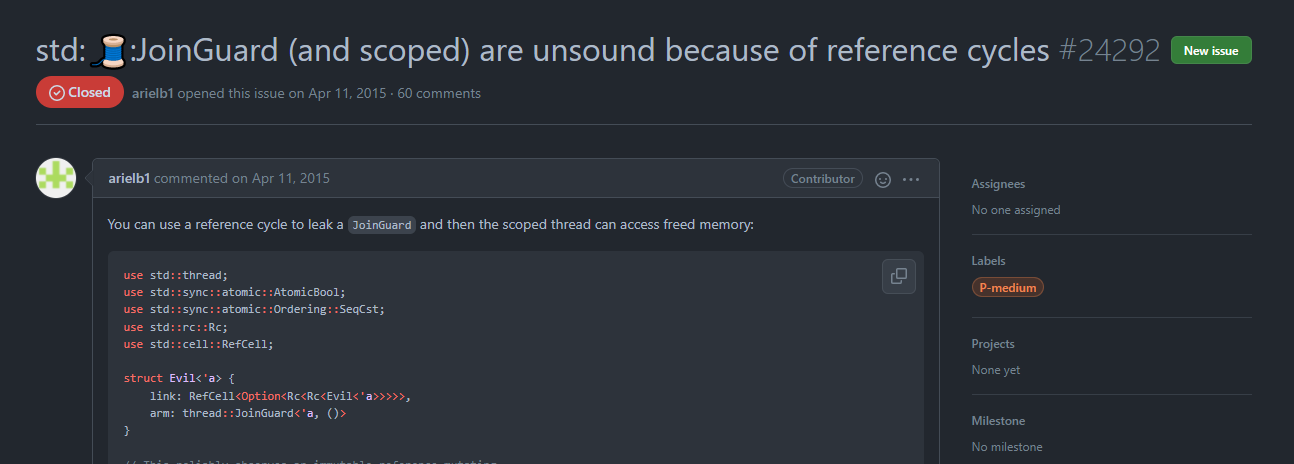
\includegraphics[width=\textwidth]{assets/thread.png}
    \caption{
\includegraphics[width=2em]{assets/thread-small.png}}
  \end{figure}

  \begin{minted}{rust}
struct Evil<'a> {
  link: RefCell<Option<Rc<Rc<Evil<'a>>>>>,
  arm: thread::JoinGuard<'a, ()>
}
  \end{minted}
\end{frame}

\begin{frame}
  \frametitle{rfcs\#1066}
  \texttt{mem::forget} 去掉了 \texttt{unsafe}.

  \pause

  \begin{itemize}
    \item \texttt{Drain} 需要确保只移出了一部分时不会访问非法内存。
    \item \texttt{Arc} 需要考虑溢出。
    \item \texttt{thread::scoped} 被完全删除了。
  \end{itemize}
\end{frame}

\begin{frame}
  \frametitle{Last but not least...}

  https://turbo.fish

  \pause

  \textbf{Bastion of The Turbofish}
  https://github.com/rust-lang/rust/blob/master/src/test/ui/bastion-of-the-turbofish.rs
\end{frame}

\begin{frame}
  \frametitle{If we got time...}

  \begin{itemize}
    \item 为什么方法里允许 \texttt{self: Pin<Self>}
    \item 为什么现在 Rust 标准库里的 HashTable 实现,在查找-插入的时候需要线性扫描两次?
    \item 为什么不能直接实现 Eq,必须得写一个 PartialEq?
    \item \texttt{impl Trait} 出现返回值、参数和别名内的意义有啥不一样?
  \end{itemize}
\end{frame}

\begin{frame}
  \frametitle{That's All!}

  \begin{center}
    
\includegraphics[width=.5\textwidth]{assets/look.png}

    Question time!
  \end{center}
\end{frame}
\end{document}
